% ============================================================
\chapter{Sensitivity Analysis}
\label{ch:sensitivity}
% ============================================================

An optimisation model is never perfect: costs, capacities, and demands are estimated, and these estimates carry margins of error. The natural question is: how far can the optimal solution remain valid if the parameters change slightly? This is the question of \emph{sensitivity analysis}, an indispensable tool for decision-makers. Thanks to the structure of the simplex and duality, one can answer this question without solving a new problem: it suffices to examine the ranges of parameter variation for which the optimal basis remains unchanged.

\section{Introduction}

In practice, the parameters of an LP (costs $c_j$, resources $b_i$,
coefficients $a_{ij}$) are never known with absolute precision.
\textbf{Sensitivity analysis} studies how the optimal solution and optimal
value change when these parameters vary.

\begin{definition}[Sensitivity analysis]
\textbf{Sensitivity analysis} (or \textbf{post-optimality analysis})
determines the ranges of parameter variation for which the \textbf{optimal
basis} remains unchanged.
\end{definition}

\section{Variation of right-hand sides $b_i$}

\subsection{Effect on the solution}

Let $\mathbf{b}' = \mathbf{b} + \Delta\mathbf{b}$.  The basic solution
becomes:
\[
  \mathbf{x}_B' = B^{-1}\mathbf{b}' = B^{-1}\mathbf{b} + B^{-1}\Delta\mathbf{b}
  = \bar{\mathbf{b}} + B^{-1}\Delta\mathbf{b}
\]

The basis remains feasible as long as $\mathbf{x}_B' \ge \mathbf{0}$:
\[
  \bar{\mathbf{b}} + B^{-1}\Delta\mathbf{b} \ge \mathbf{0}
\]

\subsection{Variation of a single $b_i$}

If only $b_i$ changes by an amount $\delta$:
\[
  \bar{b}_k + (B^{-1})_{ki} \cdot \delta \ge 0, \quad k = 1, \ldots, m
\]

\begin{keyformulas}[title=\textbf{Validity range for $b_i$}]
The basis remains optimal for:
\[
  b_i \in \left[
    b_i - \min_{k:\, (B^{-1})_{ki}>0} \frac{\bar{b}_k}{(B^{-1})_{ki}},\;
    b_i + \min_{k:\, (B^{-1})_{ki}<0} \frac{-\bar{b}_k}{(B^{-1})_{ki}}
  \right]
\]
\end{keyformulas}

\begin{theorem}[Variation of $z^*$]
When $b_i$ varies by $\delta$ within the validity range:
\[
  z^*(\delta) = z^* + y_i^* \cdot \delta
\]
where $y_i^*$ is the shadow price (dual variable) of constraint $i$.
\end{theorem}

\begin{example}[Variation of $b_1$]
Consider the LP from Chapter~3:
\[
\max\ z = 5x_1 + 4x_2 \quad \text{s.t.} \quad
6x_1 + 4x_2 \le 24,\; x_1 + 2x_2 \le 6
\]

The final tableau gives $B^{-1} = \begin{pmatrix} 1/4 & -1/2 \\
-1/8 & 3/4 \end{pmatrix}$, $\bar{\mathbf{b}} = (3, 3/2)^\top$,
$y_1^* = 3/4$, $y_2^* = 1/2$.

For variation of $b_1 = 24$:
\begin{itemize}
  \item $(B^{-1})_{11} = 1/4 > 0$: $\delta \ge -\bar{b}_1/(1/4) = -12$
  \item $(B^{-1})_{21} = -1/8 < 0$: $\delta \le -\bar{b}_2/(-1/8) = 12$
\end{itemize}
So $b_1 \in [24-12, 24+12] = [12, 36]$.

If $b_1 = 30$: $z^*(30) = 21 + (3/4)(30-24) = 21 + 4.5 = 25.5$.
\end{example}

\section{Variation of objective coefficients $c_j$}

\subsection{Basic variable}

If $x_j$ is a basic variable, changing $c_j$ affects the reduced costs of
non-basic variables.  The basis remains optimal as long as all reduced costs
remain $\ge 0$ (minimization) or $\le 0$ (maximization tableau).

\begin{keyformulas}[title=\textbf{Validity range for $c_j$ (basic variable)}]
The reduced costs of non-basic variables $k$ become:
\[
  \bar{c}_k' = \bar{c}_k - \delta \cdot \bar{a}_{rk}
\]
where $r$ is the row of $x_j$ in the basis and $\delta = c_j' - c_j$.
The basis remains optimal for $\bar{c}_k' \ge 0$ for all non-basic $k$.
\end{keyformulas}

\subsection{Non-basic variable}

If $x_j$ is non-basic with $\bar{c}_j > 0$ (maximization), the basis
remains optimal as long as $\bar{c}_j + \delta \ge 0$, i.e.,
$c_j \ge c_j - \bar{c}_j$.

\begin{example}[Variation of $c_1$]
In our example, $x_1$ is basic.  The reduced costs of non-basic variables
($s_1, s_2$) in the final tableau are:
$\bar{c}_{s_1} = 3/4$, $\bar{c}_{s_2} = 1/2$.

Row of $x_1$ gives $\bar{a}_{1,s_1} = 1/4$, $\bar{a}_{1,s_2} = -1/2$.

\begin{itemize}
  \item $\bar{c}_{s_1}' = 3/4 - \delta(1/4) \ge 0 \Rightarrow \delta \le 3$
  \item $\bar{c}_{s_2}' = 1/2 - \delta(-1/2) = 1/2 + \delta/2 \ge 0
        \Rightarrow \delta \ge -1$
\end{itemize}
So $c_1 \in [5-1, 5+3] = [4, 8]$.
\end{example}

\section{Adding a new variable}

If we add a variable $x_{n+1}$ with cost $c_{n+1}$ and technological column
$\mathbf{a}_{n+1}$, compute:
\[
  \bar{c}_{n+1} = c_{n+1} - \mathbf{c}_B^\top B^{-1} \mathbf{a}_{n+1}
\]

\begin{itemize}
  \item If $\bar{c}_{n+1} \ge 0$ (minimization): the solution remains
        optimal without using $x_{n+1}$.
  \item If $\bar{c}_{n+1} < 0$: it is beneficial to bring $x_{n+1}$ into
        the basis.
\end{itemize}

\section{Adding a new constraint}

If we add a constraint $\mathbf{a}_{m+1}^\top \mathbf{x} \le b_{m+1}$:
\begin{enumerate}
  \item Check whether the current optimal solution $\mathbf{x}^*$ satisfies
        the new constraint: $\mathbf{a}_{m+1}^\top \mathbf{x}^* \le b_{m+1}$.
  \item If yes: the solution remains optimal.
  \item If no: apply the \textbf{dual simplex} by adding the constraint
        (with a slack variable) to the final tableau.
\end{enumerate}

\section{Parametric analysis}

\begin{definition}[Parametric analysis]
\textbf{Parametric analysis} studies the continuous variation of $z^*$ as a
function of a parameter $\theta$:
\[
  \mathbf{b}(\theta) = \mathbf{b} + \theta \mathbf{d}
  \qquad \text{or} \qquad
  \mathbf{c}(\theta) = \mathbf{c} + \theta \mathbf{e}
\]
where $\mathbf{d}$ or $\mathbf{e}$ are fixed directions.
\end{definition}

\begin{theorem}[Shape of $z^*(\theta)$]
The optimal value $z^*(\theta)$ is a \textbf{piecewise linear} and
\textbf{concave} function (when varying $\mathbf{b}$ in a maximization
problem) of $\theta$.  Each segment corresponds to a different optimal basis.
\end{theorem}

\begin{center}
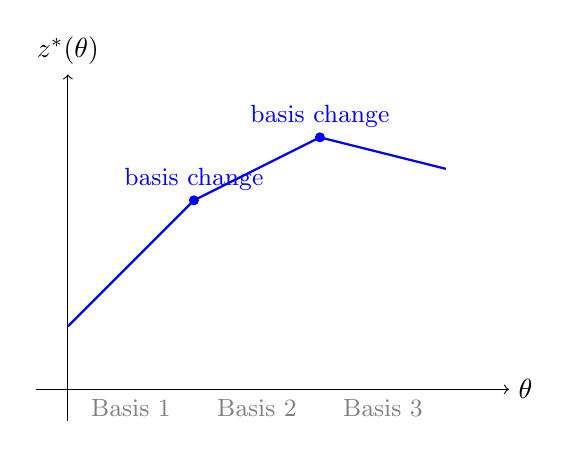
\begin{tikzpicture}[scale=0.8]
  \draw[->] (-0.5,0) -- (7,0) node[right] {$\theta$};
  \draw[->] (0,-0.5) -- (0,5) node[above] {$z^*(\theta)$};
  \draw[thick, blue] (0,1) -- (2,3) -- (4,4) -- (6,3.5);
  \filldraw[blue] (2,3) circle (2pt) node[above] {\small basis change};
  \filldraw[blue] (4,4) circle (2pt) node[above] {\small basis change};
  \node[gray, below] at (1,0) {\small Basis 1};
  \node[gray, below] at (3,0) {\small Basis 2};
  \node[gray, below] at (5,0) {\small Basis 3};
\end{tikzpicture}
\end{center}

\section{Python implementation}

\begin{codeblock}[title=\textbf{Sensitivity analysis with SciPy}]
\begin{minted}{python}
from scipy.optimize import linprog
import numpy as np

c = [-5, -4]  # max 5x1 + 4x2
A_ub = [[6, 4], [1, 2]]
b_ub = [24, 6]
bounds = [(0, None), (0, None)]

# Base solution
res = linprog(c, A_ub=A_ub, b_ub=b_ub, bounds=bounds,
              method='highs')
print(f"z* = {-res.fun:.2f}, x* = {res.x}")

# Sensitivity on b1
print("\nVariation of b1:")
for delta in [-12, -6, 0, 6, 12]:
    b_new = [24 + delta, 6]
    r = linprog(c, A_ub=A_ub, b_ub=b_new, bounds=bounds,
                method='highs')
    print(f"  b1={24+delta:3d} -> z*={-r.fun:.2f}, "
          f"x*=[{r.x[0]:.2f}, {r.x[1]:.2f}]")

# Sensitivity on c1
print("\nVariation of c1:")
for c1 in [3, 4, 5, 6, 8]:
    c_new = [-c1, -4]
    r = linprog(c_new, A_ub=A_ub, b_ub=b_ub, bounds=bounds,
                method='highs')
    print(f"  c1={c1} -> z*={-r.fun:.2f}, "
          f"x*=[{r.x[0]:.2f}, {r.x[1]:.2f}]")
\end{minted}
\end{codeblock}

\begin{codeoutput}
z* = 21.00, x* = [3.  1.5]

Variation of b1:
  b1= 12 -> z*= 12.00, x*=[0.00, 3.00]
  b1= 18 -> z*= 16.50, x*=[1.50, 2.25]
  b1= 24 -> z*= 21.00, x*=[3.00, 1.50]
  b1= 30 -> z*= 25.50, x*=[4.50, 0.75]
  b1= 36 -> z*= 30.00, x*=[6.00, 0.00]

Variation of c1:
  c1=3 -> z*= 15.00, x*=[3.00, 1.50]
  c1=4 -> z*= 18.00, x*=[3.00, 1.50]
  c1=5 -> z*= 21.00, x*=[3.00, 1.50]
  c1=6 -> z*= 24.00, x*=[3.00, 1.50]
  c1=8 -> z*= 30.00, x*=[3.00, 1.50]
\end{codeoutput}

\section{Sensitivity report}

Commercial solvers provide a \textbf{sensitivity report} containing for each
constraint and variable:

\begin{center}
\renewcommand{\arraystretch}{1.2}
\begin{tabular}{lp{8cm}}
  \toprule
  \textbf{Information} & \textbf{Description} \\
  \midrule
  Optimal value & Value of the variable/constraint at optimality \\
  Shadow price & Marginal change in $z^*$ per unit of $b_i$ \\
  Reduced cost & Marginal change in $c_j$ needed for $x_j$ to enter
                  the basis \\
  Allowable increase & Upper bound on variation \\
  Allowable decrease & Lower bound on variation \\
  \bottomrule
\end{tabular}
\end{center}

\section{Exercises}

\begin{exercise}[$\star$ --- Validity ranges]
For the LP:
\[
\max\ z = 3x_1 + 2x_2 \quad \text{s.t.} \quad
x_1 + x_2 \le 10,\; 2x_1 + x_2 \le 14,\; x_1, x_2 \ge 0
\]
Determine the validity ranges for $b_1$ and $b_2$.
\end{exercise}

\begin{exercise}[$\star\star$ --- Objective variation]
For the same LP, determine the range of $c_1$ for which the optimal basis
does not change.
\end{exercise}

\begin{exercise}[$\star\star$ --- New variable]
Should we introduce a new product $P_3$ with profit $c_3 = 6$ and resource
consumption $(a_{13}, a_{23}) = (3, 1)$?
\end{exercise}

\begin{exercise}[$\star\star$ --- New constraint]
Add the constraint $x_1 + x_2 \le 5$.  Is the optimal solution still
feasible?  If not, find the new optimal solution.
\end{exercise}

\begin{exercise}[$\star\star\star$ --- Complete parametric analysis]
Study $z^*(\theta)$ for $\mathbf{b}(\theta) = (10 + \theta, 14 - 2\theta)$
as $\theta$ varies from $-5$ to $+5$.  Plot the curve and identify basis
changes.
\end{exercise}

\begin{exercise}[$\star\star\star$ --- Implementation]
Write a Python script that:
\begin{enumerate}
  \item Solves an LP with PuLP.
  \item Automatically computes validity ranges for each $b_i$ via numerical
        perturbation.
  \item Plots $z^*(\theta)$ for a parametric variation of $b_1$.
\end{enumerate}
\end{exercise}
